Theoretically an IRT fact split and matching text set are sufficient for training the Power model. However, when evaluat However, when evaluating the trained model against the IRT split's open-world entities, Power would perform only mediocre as it could only use its Texter component for inference, since the open-world entities do not provide any facts the Ruler can work with. Therefore, considering the intended few-shot scenario, the IRT splits are transformed to \emph{Power splits}, that involve some known facts for the test entities, by dividing the IRT split's open-world facts into so-called \emph{known facts}, that are allowed to be used for rule application during inference, and \emph{unknown facts}, that stay unknown. Meanwhile, the close-world entities' training and validation facts are merged as there is no need for the latter. Figure~\ref{fig:5_experiments/2_power_datasets/splits} illustrates the repartitioning.

\begin{figure}[t]
    \centering
    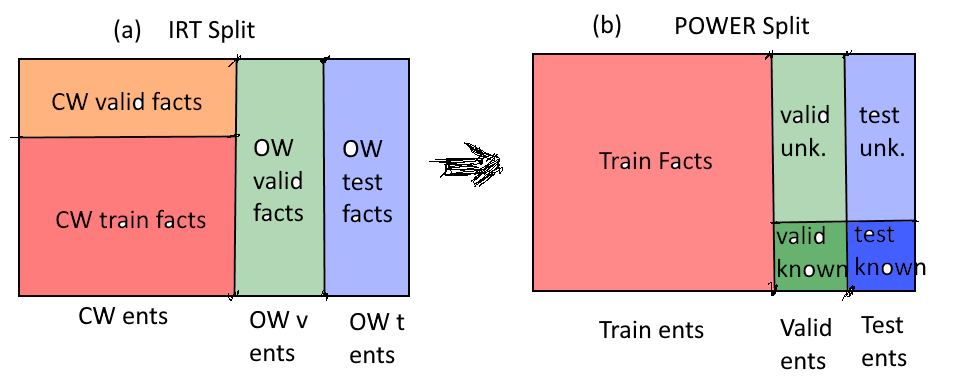
\includegraphics[width=\textwidth]{5_experiments/2_power_datasets/splits}
    \caption{Repartitioning an IRT fact split into a Power split by merging the train subsets and splitting validation and test subsets into facts are known and unknown during inference, respectively}
    \label{fig:5_experiments/2_power_datasets/splits}
\end{figure}

The percentage of known and unknown facts can be varied when creating the Power split to study the Ruler's effectiveness on entities with more or less given knowledge. Table~\ref{tab:5_experiments/2_power_datasets/power_splits} lists the splits used for the evaluation. In practice, few-shot splits are particularly interesting. Since there are only about 20 facts per entity on average, the fact splits with 5\% and 15\% known facts can be considered few-shot scenarios. The splits with 0\% known facts correspond to an zero-shot open-world scenario. For readability, the Power splits based on the CoDEx-M and FB15k-237 splits are abbreviate to "CDE" and "FB".

\begin{table}[h]
    \centering
    \begin{tabular}{| l | r | r | r | r | r |}
    \hline
    
    \multicolumn{1}{|c|}{\textbf{Power Split}} &
    \multicolumn{1}{|c|}{\textbf{\thead{Train Facts}}} &
    \multicolumn{1}{|c|}{\textbf{\thead{Known \\ Valid Facts}}} &
    \multicolumn{1}{|c|}{\textbf{\thead{Known \\ Valid Facts \\ per Entity}}} &
    \multicolumn{1}{|c|}{\textbf{\thead{Known \\ Test Facts}}} &
    \multicolumn{1}{|c|}{\textbf{\thead{Known \\ Test Facts \\ per Entity}}} \\

    \hline\hline

    CDE-0   & \multirow{6}{*}{\num{137738}} & \num{0}     & \num{0.00} & \num{0}     & \num{0.00} \\
    CDE-5   &                               & \num{2062}  & \num{0.71} & \num{1378}  & \num{0.73} \\
    CDE-15  &                               & \num{6186}  & \num{2.12} & \num{4136}  & \num{2.18} \\
    CDE-30  &                               & \num{12372} & \num{4.24} & \num{8273}  & \num{4.36} \\
    CDE-50  &                               & \num{20620} & \num{7.07} & \num{13788} & \num{7.27} \\
    CDE-100 &                               & \num{?}     & \num{7.07} & \num{13788} & \num{7.27} \\

    \hline

    FB-0   & \multirow{6}{*}{\num{238191}} & \num{0}     & \num{0.00}  & \num{0}     & \num{0.0} \\
    FB-5   &                               & \num{2325}  & \num{1.50}  & \num{1271}  & \num{1.56} \\
    FB-15  &                               & \num{6975}  & \num{4.51}  & \num{3813}  & \num{4.67} \\
    FB-30  &                               & \num{13950} & \num{9.03}  & \num{7626}  & \num{9.35} \\
    FB-50  &                               & \num{23251} & \num{15.05} & \num{12711} & \num{15.58} \\
    FB-100 &                               & \num{?}     & \num{15.05} & \num{12711} & \num{15.58} \\
    
    \hline
\end{tabular}

    \caption{Power splits with varying ratios of known test entities - for example, "CDE-50" denotes the CoDEx-M-based Power split with half of the test entities being known during inference while the FB-0 Power split does not reveal any of the FB15k-237 facts during inference}
    \label{tab:5_experiments/2_power_datasets/power_splits}
\end{table}
